\documentclass[a4paper, oneside, 12pt]{report}
\usepackage[slovene]{babel}
\usepackage[utf8]{inputenc}
\usepackage[left=3cm, top=3cm, right=2.5cm, bottom=2.5cm]{geometry}
\usepackage{fancyhdr}
\usepackage{etoolbox}
\usepackage{graphicx}
\usepackage{tabulary}

% TOC.
\usepackage[nottoc]{tocbibind}
\usepackage{tocloft}
\tocloftpagestyle{fancy}

% Rename things.
\addto\captionsslovene{
	\renewcommand{\contentsname}{Kazalo vsebine}
	\renewcommand{\listfigurename}{Kazalo slik}
	\renewcommand{\listtablename}{Kazalo preglednic}
%	\renewcommand{\listappendicesname}{Kazalo prilog}
}

% Change chapter formatting.
\makeatletter
\def\@makechapterhead#1{
	\vspace*{30\p@}
	{\noindent\Huge\bf\thechapter \hspace*{0.5cm} \parindent \z@ \raggedright \normalfont
		\interlinepenalty\@M
		\Huge \bfseries #1\par\nobreak
		\vskip 30\p@
	}
}
\def\@makeschapterhead#1{
	\vspace*{30\p@}
	{\noindent\Huge\bf \parindent \z@ \raggedright \normalfont
		\interlinepenalty\@M
		\Huge \bfseries #1\par\nobreak
		\vskip 30\p@
	}
}
\makeatother

% Priloge.
%\usepackage{appendix}
%\addto\captionsslovene{
%	\renewcommand\appendixname{Priloga}
%	\renewcommand\appendixpagename{Priloge}
%}

% Kazalo prilog.
%\usepackage{tocloft}
%\newcommand{\listappendicesname}{Priloge}
%\newlistof{appendices}{apc}{\listappendicesname}
%\renewcommand{\appendices}[1]{\addcontentsline{apc}{appendices}{#1}}

% Seznam kratic.
\usepackage{longtable}
\newcommand\nomenclature[2]{#1 & #2 \\}

% Backreference.
\usepackage[pageref]{backref}
\usepackage{url}
\def\backreftwosep{ in~}
\def\backreflastsep{ in~}
\renewcommand*{\backref}[1]{}
\renewcommand*{\backrefalt}[4]{
	\ifcase #1 {\it (Ni citirano.)}
	\or        {\it (Citirano na strani~#2.)}
	\else      {\it (Citirano na straneh~#2.)}
	\fi}

%% To Do
% Read Reinforcement Learning: A Survey.
% Read Deepming research paper.
% Set up github, CC licence.

%% Alternative Titles
% Strojno učenje: učenje iz interakcije
% Strojno učenje: učenje z interakcijo
% Strojno učenje: okrepitveno učenje
% Strojno učenje z interakcijo z okoljem
% Strojno učenje v neznanem okolju
% Strojno učenje s poizkušanjem
% Strojno učenje na podlagi izkušenj
% Machine learning from trial-and-error

\pagestyle{fancy}
\fontfamily{timesnewroman}
\linespread{1.25}

\lhead{\footnotesize Breulj R. Strojno učenje iz interakcije
\\Univerza na Primorskem, FAMNIT, 2014}
\rhead{\thepage}
\cfoot{}
\setlength{\headheight}{24pt}

\begin{document}
\begin{titlepage}
\begin{center}
\begin{large}
UNIVERZA NA PRIMORSKEM\\
FAKULTETA ZA MATEMATIKO, NARAVOSLOVJE IN\\
INFORMACIJSKE TEHNOLOGIJE\\[6cm]
\end{large}
\end{center}

\begin{center}
Zaključna naloga\\
\textbf{\large Strojno učenje iz interakcije}\\
Machine learning from interaction\\[6cm]
\end{center}

\noindent
Ime in priimek: Rok Breulj\\
Študijski program: Računalništvo in informatika\\
Mentor: doc. dr. Peter Rogelj\\

\vfill
\begin{center}
{\large Koper, Avgust 2014}
\end{center}
\end{titlepage}

\pagenumbering{roman}

\section*{Ključna dokumentacijska informacija}
\medskip
\begin{center}
\fbox{\parbox{\linewidth}{
\vspace{0.2cm}
\noindent
Ime in PRIIMEK:\vspace{0.5cm}\\
Naslov zaključne naloge:\vspace{0.5cm}\\
Kraj:\vspace{0.5cm}\\
Leto:\vspace{0.5cm}\\
Število listov: \hspace{2cm} Število slik: \hspace{2.6cm} Število tabel:\hspace{2cm}\vspace{0.5cm}\\
Število prilog: \hspace{1.9cm} Število strani prilog: \hspace{1cm} Število referenc:\vspace{0.5cm}\\
Mentor:\vspace{0.5cm}\\
Somentor:\vspace{0.5cm}\\
Ključne besede:\vspace{0.5cm}\\
Math.~Subj.~Class.~(2010):\vspace{0.5cm}\\
{\bf Izvleček:}\\
Izvleček predstavlja kratek, a jedrnat prikaz vsebine naloge. V največ 250 besedah nakažemo problem, metode, rezultate, ključne ugotovitve in njihov pomen.
\vspace{0.2cm}
}}
\end{center}
\newpage

\section*{Key words documentation}
\medskip
\begin{center}
\fbox{\parbox{\linewidth}{
\vspace{0.2cm}
\noindent
Name and SURNAME:\vspace{0.5cm}\\
Title of final project paper:\vspace{0.5cm}\\
Place:\vspace{0.5cm}\\
Year:\vspace{0.5cm}\\
Number of pages:\hspace{1.6cm} Number of figures:\hspace{2.2cm} Number of tables:\vspace{0.5cm}\\
Number of appendices:\hspace{0.6cm} Number of appendix pages:\hspace{0.8cm}Number of references:\vspace{0.5cm}\\
Mentor:\vspace{0.5cm}\\
Co-Mentor:\vspace{0.5cm}\\
Keywords:\vspace{0.5cm}\\
Math.~Subj.~Class.~(2010):\vspace{0.5cm}\\
{\bf Abstract:}
\vspace{0.2cm}
}}
\end{center}
\newpage

\section*{Zahvala}
%Preface? Foreword?
% I was looking for a way to learn without prior knowledge of the problem. A universal learner.
% Reinforcement learning is one way -- trial and error interaction with the environment
% Observation (of the correct approach) is another, faster way of getting it right
% Teaching is the fastest way -- supervised learning
%In 1959, Arthur Samuel defined machine learning as a “Field of study that gives computers the ability to learn without being explicitly programmed”
% No one single learning way is best for everything, teaching is generally the fastest, but exercise and experiments afterwards are needed to absorb and enforce the knowledge.
\newpage

\tableofcontents
\thispagestyle{fancy}
\newpage

\listoftables
\thispagestyle{fancy}
\newpage

\listoffigures
\thispagestyle{fancy}
\newpage

%\listofappendices
%\thispagestyle{fancy}
%\addcontentsline{toc}{chapter}{Seznam prilog}
%\newpage

\chapter*{Seznam kratic}
\addcontentsline{toc}{chapter}{Seznam kratic}
\thispagestyle{fancy}
\begin{longtable}{@{}p{1cm}@{}p{\dimexpr\textwidth-1cm\relax}@{}}
\nomenclature{$tj.$}{to je}
\nomenclature{$npr.$}{na primer}
\end{longtable}
\newpage

\pagenumbering{arabic}

\chapter{Uvod}
\thispagestyle{fancy}
% learning, interaction, no teacher, environment, trial and error, influence through behavior, environment responds (input), intelligence, draw conclusions
Učimo se skozi naše celotno življenje. En od osnovnih načinov učenja temelji na podlagi interakcije z okoljem. V računalništvu velikokrat radi odidemo po tej eksperimentalni poti, posebej ko verjamemo, da smo blizu rešitvi. Ampak ni potrebno pogledati tako daleč kot je računalništvo. Že kot otroci, ko mahamo z rokami in gledamo naokoli, nimamo izrecnega učitelja, imamo pa neposredno senzomotorično povezavo z našo okolico. S svojim vedenjem vplivamo na okolje in naša čutila izkoriščamo za pridobitev ogromne količine podatkov o vzrokih in učinkih, o posledicah dejanj in kako doseči cilje. Skozi naše življenje so takšne interakcije nedvoumno velik izvir znanja o našem okolju in samih sebe. Ko se učimo voziti avto ali pogovarjati, se zavedamo kako se okolje odziva na naša dejanja in iščemo način kako vplivati na rezultat z našim vedenjem.
%Ideja učenja iz interakcije z našim okoljem je ena od prvih, ki nam pride na misel, ko razmišljamo o naravi učenja. Ko se dojenček igra, maha z rokami ali gleda naokoli nima izrecnega učitelja, ima pa neposredno senzomotorično povezavo z okoljem. Uporaba te povezave proizvede ogromno informacije o vzrokih in učinkih, o posledicah dejanj in načinih kako doseči cilje. Skozi naše življenje so takšne interakcije nedvoumno velik izvir znanja o našem okolju in samih sebe. Ko se učimo voziti avto ali pogovarjati, se zavedamo kako se okolje odziva na naša dejanja in iščemo način kako vplivati na rezultat z našim vedenjem.~\cite{Intro}
%Learning from interaction is a foundational idea underlying nearly all theories of learning and intelligence.

% capable of surviving in a new environment, adapt an appropriate behavior, evaluate and classify new situations
% Intelligence measures an agent’s ability to achieve goals in a wide range of environments.” S. Legg and M. Hutter
Čeprav ni ene same standardne definicije inteligence, lahko primerjamo zbirko predlaganih definicij med seboj in hitro najdemo močne podobnosti med njimi. V veliko primerih, definicije inteligence vsebuje idejo, da se posameznik, ki je inteligenten, mora znati prilagoditi okoljem, ki jih ni še nikdar srečal, in v njih doseči cilje~\cite{ACollectionOfDefinitionsOfIntelligence}. Za inteligentno obnašanje očitno torej potrebujemo način, da ovrednotimo in razvrstimo nove položaje. Da se posameznik lahko uči in prilagodi svoje obnašanje, mora znati upoštevati tudi informacije iz okolja in iz njih sklepati. Okrepitveno učenje (angl. reinforcement learning) predstavlja teorijo o učenju povečanja nagrade na voljo v okolici in tako neposredno povečanje možnosti prilagoditve in preživetja. Nekatere naloge so preveč zapletene za jih opisati v statičnem računalniškem programu, kar je danes pogost postopek. Način za dinamično učenje in razvijanje programa je za nekatere naloge torej potreben.

% intelligent systems, dynamic real-world environments, autonomous, not relying on controlled conditions, uncertainty, time constrants, decision making, under these conditions reinforcement learning can have considerate advantages over other types of learning
Praktično vse kar živali, podjetja in računalniški programi delajo vključuje niz dejanj za dosego cilja. Ali je to vožnja avta do dela ali priprava jutranje kave, obstaja cilj in zaporedje dejanj za uspešno opravljen cilj. Prilagodljiv krmilni sistem, ki se zna učiti izvajati takšne sekvenčne naloge odločanja lahko najde vlogo v številnih domenah, kot so krmiljenje proizvodnega procesa, avtonomnih vozilih, letalstvu in pripomočkih za invalide. V pametnih sistemih, ki delujejo v dinamičnih okoljih resničnega sveta, kjer se ne moremo zanašati nad nadzorljivimi pogoji, kjer veljajo negotovost in časovne omejitve, ima lahko odločanje na podlagi okrepitvenega učenja obzirne prednosti pred ostalimi vrstami učenja.

% multi-disciplinary field: ai, psychology, control engineering, operations research, neuroscience, artificial neural networks, genetic algorithms
Področje okrepitvenega učenja je zelo interdisciplinarno, z močnimi vezami v teoriji krmiljenja (angl. control theory), psihologiji in nevroznanosti. Teorija krmiljenja pripomore k rešitvi problema z analitičnega, matematičnega vidika, med tem ko se psihologija in nevroznanost zgledujeta po bioloških procesih za odgovore. Veliko temeljnih smernic je izpeljanih iz psihologije vedenja in učenja; teorijah, ki se tičejo nagrajevanja in pogojevanja dejanj. Algoritmični pristopi so speljani pod podobnimi principi kot ljudje in živali oblikujemo vedenja glede na odzive iz okolice.

% past work
Zamisel o gradnji inteligentni strojev dolgo navdušuje človeštvo; že egipčani so o tem razmišljali. Čez leta se je razvilo veliko teorij, ampak komaj z uvodom modernega računalnika, 60 let nazaj, se je umetna inteligenca in strojno učenje razvilo v svojo znanstveno področje~\cite{TDANNForStrategicControlProblems}. Leta 1948 je Claude Elwood Shannon~\cite{AMathematicalTheoryOfCommunication} napisal predlog za šahovski program in leta 1959 je Arthur Samuel~\cite{SomeStudiesInMachineLearningUsingTheGameOfCheckers} razvil računalniški program, ki se je naučil igrati namizno igro dama z igranjem proti samemu sebi. V zadnjih letih so se raziskave osredotočale bolj na posnemanje bioloških modelov v poizkušanju izdelave programov, ki rešujejo probleme in razmišljajo kot ljudje. Nevrološke mreže (angl. neural networks), zelo poenostavljen model možganov, so bile uspešno uporabljene v vrsti aplikacijah. Po formalizaciji Samuelevega pristopa in oblikovanja učenja na podlagi časovne razlike lambda Richarda Suttona~\cite{LearningToPredictByTheMethodsOfTemporalDifference}, je v 1992 Richard Tesauro~\cite{PracticalIssuesInTemporalDifferenceLearning} razvil Backgammon igralca, ki je tekmoval proti najboljšim človeškim igralcem na svetu. Čeprav je Tesaurova združitev pristopa okrepitvenega učenja in nevroloških mrež pretresla področje umetne inteligence in Backgammon skupnosti, ni bilo veliko drugih uspehov v namiznih igrah~\cite{PlayingRiskAversiveGoOnALargeBoardUsingLocalNeuralNetworkPositionEvaluationFunctions, StrategyAcquisitionForTheGameOthelloBasedOnReinforcementLearning, LearningToEvaluateGoPositionsViaTemporalDifferenceMethods}. Prenos Tesaurove rešitve v največje namizne igre v področju umetne inteligence, šah in Go, niso uspele; rezultati so bili slabši kot so jih dosegle konvencionalne metode. Poleg namiznih iger je bilo okrepitveno učenje uporabljeno tudi v problemih robotike, razporejanja, dinamičnih dodelitev in optimizacije~\cite{ReinforcementLearningAnIntroduction}.

% 10000 hours to master skill, 20 hours to acquire new skill
% brain energy consumption and comparison to other primate and rodent brains -- we have the largest number of neurons in the cerebral cortex, and are the only ones that cook, allowing us to intake the energy needed to sustain the amount of neurons and the size of our body: https://www.youtube.com/watch?v=_7_XH1CBzGw
% Learning rate <-> human age.

% what's in this work
% computational approach, learning methods, ai, goal-directed learning from interaction, other approaches to machine learning
% reinforcement learning from the view of ai and engineering (not psychology or neuroscience)
% mathematical forumlation of learning from interaction
% unified notation
% how the different algorithms are related and combine, combinations 
% games are sequential decisions tasks, provide convenient testbeds for the study of such learning
% their goals and rules are well defined simplifying the modeling and simulation process
% at the same time, the problem they present are both challenging and interesting
% Hex
%Skozi implementacijo namizne igre Hex v nalogi raziščem okrepitveno učenje (angl. reinforcement learning), področje strojnega učenja, ki se ukvarja z vprašanjem kako se vesti v neznanem okolju, da bi povečali številčni nagrajevalni signal. Okrepitveno učenje se razlikuje od nadzorovanega učenja v tem, da nam niso nikoli prikazana pravilna dejanja ali pa napačna popravljena. Poudarek je tudi na zmogljivosti učenja med izvedbo, katero pelje do iskanja ravnovesja med raziskovanjem neznanih stanj in izkoriščanjem obstoječega znanja. Ukvarja se s celotnim problemom učenja iz interakcije z neznanim okoljem.
V nadaljevanju naloge je pregledan izvor okrepitvenega učenja iz vedenjske plati v razdelku~\ref{section:Psychology}. Nato je zavzet pogled iz strani umetne inteligence in inženirstva. Raziščen je računski pristop do učenja iz interakcije. V razdelku~\ref{section:} je matematično definiran celoten problem okrepitvenega učenja in v razdelku~\ref{section:} so predstavljene rešitve. Primerjani so različni algoritmi, njihove povezave in kombinacije. Ker imajo abstraktne namizne igre dobro definirane cilje in pravila, kar poenostavi model in simulacijo, in hkrati predstavljajo izziven in zanimiv problem, so priročno testno okolje za študijo takšnega učenja. 
V razdelku~\ref{} so rešitve iz okrepitvenega učenja uporabljene v namizni igri Hex in na koncu v razdelku~\ref{} razpravljeni rezultati skupaj s pogledom na prihodnost.
% cilj, originalnost dela je v aplikaciji okrepitvenega učenja na Hex igro

\section{Psihologija} \label{section:Psychology}
% https://new.edu/nodes/learning-and-behavior
% roots psychology of animal learning, where it takes its name
% dog clicker (=classical conditioning), dog training (=classical conditioning+operant for orders), people and animal learning
% psychology, operant conditioning (reinforcement), classical conditioning (association), (other non-related: observational learning)
% operant is for control, it affects the environment
% classical is for prediction, it does not affect the environment
% http://www.oxfordbibliographies.com/view/document/obo-9780199828340/obo-9780199828340-0043.xml
% Mazur, J. E. 2006. Learning and behavior. 6th ed. Upper Saddle River, NJ: Pearson Prentice Hall.
Okrepitveno učenje ima korenine v psihologiji učenja živali, iz kjer izvira tudi samo ime. Posebej se nanaša na klasično pogojevanje (angl. classical conditioning) in operantno pogojevaje (angl. operant conditioning).

\subsection{Klasično pogojevanje}
Klasično pogojevanje (imenovana tudi Pavlovo pogojevanje) je učenje prek povezav oz. asociacij.

V začetku 20. stoletja je ruski psiholog Ivan Pavlov (1849-1936) med preučevanjem prebavnega sistema psov odkril vedenjski fenomen~\cite{ConditionedReflexes}: psi so se začeli sliniti, ko so laboratorijski tehniki, ki so jih hranili, vstopili v sobo; čeprav psi še niso dobili hrane. Pavlov je spoznal, da so se psi začeli sliniti, ker so vedeli, da bodo nahranjeni; povezali so prihod tehnikov s hranjenjem.

S svojo ekipo je pričel raziskovati proces bolj podrobno. Izvedel je serijo eksperimentov v katerih so bili psi izpostavljeni zvoku trenutek preden so dobili hrano. Sistematično je nadzoroval časovno razliko med pojavom zvoka in hrano in zabeležil količino sline pri pseh. Najprej so se psi slinili samo, ko so videli ali zavohali hrano. Po večkratnem predstavljenem zvoku skupaj s hrano pa so se psi začeli sliniti takoj, ko so zaslišali zvok. Naučili so se povezave med zvokom in hrano, ki je sledila.

Pavlov je odkril temeljni asociativni proces imenovan klasično pogojevanje; učenje, ki se pojavi, ko nevtralna spodbuda (na primer: zvok) postane povezana s spodbudo, ki sama po sebi naravno proizvede vedenje (na primer: hrana). Po tem, ko je povezava naučena, predhodno nevtralna spodbuda zadošča za proizvedbo vedenja, ki je večinoma enakovredno (Pavlov je opazil razliko v sestavi sline~\cite{PavlovianConditioningItsNotWhatYouThinkItIs, LearningAndBehaviorAContemporarySynthesis, CognitionEvolutionAndBehavior}).

Prihod tehnikov oz. zvok je Pavlov imenoval pogojena spodbuda (angl. conditioned stimulus CS), ker je njen učinek odvisen od povezave s hrano. Hrano je imenoval nepogojena spodbuda (angl. unconditioned stimulus US), ker njen učinek ni odvisen od predhodnih izkušenj. Podobno je pogojen odziv (angl. conditioned response CR) odziv pogojene spodbude CS in nepogojen odziv (angl. unconditioned response UR) odziv nepogojene spodbude US. Pavlov je odkril, da je krajši razmak med zvokom in prikazom hrane povzročil močnejše in hitrejše učenje pogojenega odziva CR psa~\cite{PsychologyAStudentFriendlyApproach}.

% Make it black and white to fit the style of the rest?
\begin{figure}[htbp]
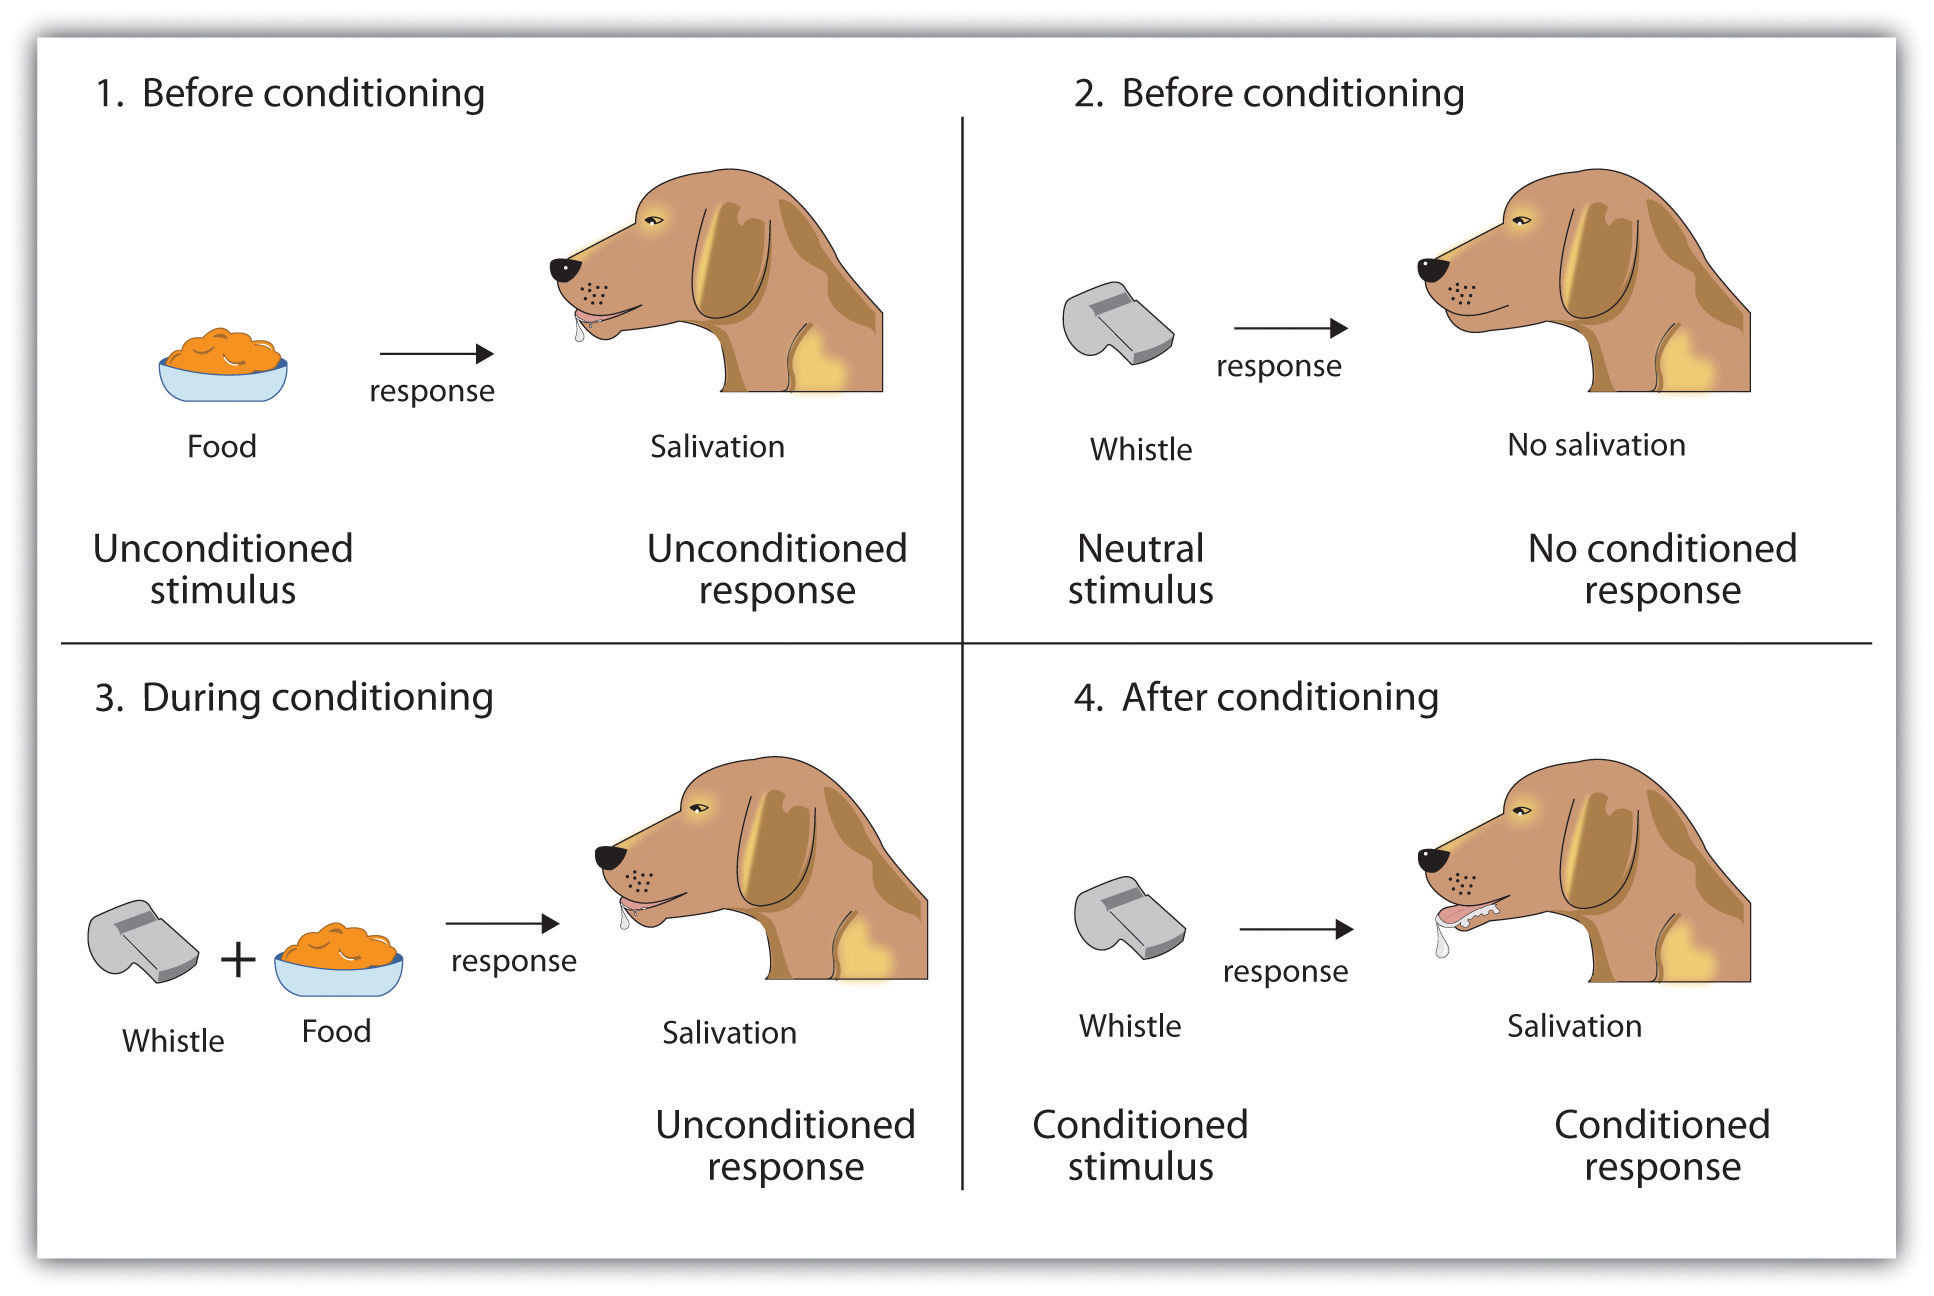
\includegraphics[scale=0.226]{WhistleAndDog.jpg}
\caption{Klasično pogojevanje piščalke namesto hrane za slinjenje pri psu~\cite{IntroductionToPsychology}.}
\label{figure:WhistleAndDog}
\end{figure}

Pogojevanje je evolucijsko koristno, ker omogoča organizmom razviti pričakovanja, ki jim pomagajo pri dobrih in slabih dogodkih. Razvidno je na primeru živali, ki zavoha novo hrano, jo poje in postane bolna. Če se žival zna naučiti povezave z vonjem (CS) in hrano (US), se bo znala izogibati določeni hrani že po vonju.

% After he had demonstrated that learning could occur through association, Pavlov moved on to study the variables that influenced the strength and the persistence of conditioning. In some studies, after the conditioning had taken place, Pavlov presented the sound repeatedly but without presenting the food afterward. Figure 7.4, “Acquisition, Extinction, and Spontaneous Recovery” shows what happened. As you can see, after the intial acquisition (learning) phase in which the conditioning occurred, when the CS was then presented alone, the behavior rapidly decreased—the dogs salivated less and less to the sound, and eventually the sound did not elicit salivation at all. Extinction refers to the reduction in responding that occurs when the conditioned stimulus is presented repeatedly without the unconditioned stimulus.

% Although at the end of the first extinction period the CS was no longer producing salivation, the effects of conditioning had not entirely disappeared. Pavlov found that, after a pause, sounding the tone again elicited salivation, although to a lesser extent than before extinction took place. The increase in responding to the CS following a pause after extinction is known as spontaneous recovery. When Pavlov again presented the CS alone, the behavior again showed extinction until it disappeared again.

% Although the behavior has disappeared, extinction is never complete. If conditioning is again attempted, the animal will learn the new associations much faster than it did the first time.

% Pavlov also experimented with presenting new stimuli that were similar, but not identical to, the original conditioned stimulus. For instance, if the dog had been conditioned to being scratched before the food arrived, the stimulus would be changed to being rubbed rather than scratched. He found that the dogs also salivated upon experiencing the similar stimulus, a process known as generalization. Generalization refers to the tendency to respond to stimuli that resemble the original conditioned stimulus. The ability to generalize has important evolutionary significance. If we eat some red berries and they make us sick, it would be a good idea to think twice before we eat some purple berries. Although the berries are not exactly the same, they nevertheless are similar and may have the same negative properties.

% The flip side of generalization is discrimination—the tendency to respond differently to stimuli that are similar but not identical. Pavlov’s dogs quickly learned, for example, to salivate when they heard the specific tone that had preceded food, but not upon hearing similar tones that had never been associated with food. Discrimination is also useful—if we do try the purple berries, and if they do not make us sick, we will be able to make the distinction in the future. And we can learn that although the two people in our class, Courtney and Sarah, may look a lot alike, they are nevertheless different people with different personalities.

% In some cases, an existing conditioned stimulus can serve as an unconditioned stimulus for a pairing with a new conditioned stimulus—a process known as second-order conditioning. In one of Pavlov’s studies, for instance, he first conditioned the dogs to salivate to a sound, and then repeatedly paired a new CS, a black square, with the sound. Eventually he found that the dogs would salivate at the sight of the black square alone, even though it had never been directly associated with the food. Secondary conditioners in everyday life include our attractions to things that stand for or remind us of something else, such as when we feel good on a Friday because it has become associated with the paycheck that we receive on that day, which itself is a conditioned stimulus for the pleasures that the paycheck buys us.

Klasično pogojevanje obravnava samo problem napovedovanja, ker odziv živali ne vpliva na eksperiment, oziroma, bolj splošno, ne vpliva na okolje. Učenje na podlagi časovne razlike (angl. temporal difference learning), opisano pozneje v razdelku~\ref{subsection:TD0Prediction}, je bilo prvotno predvsem povezano s klasičnim pogojevanjem in problemom napovedovanja, kjer pogojena spodbuda (CS) povezana s poznejšo nepogojeno spodbudo (US) povzroči potrebo po ovrednotenju časovne razlike vrednostne funkcije. Cilj izračuna je zagotoviti, da po učenju pogojena spodbuda (CS) postane napovednik nepogojene spodbude (US). Kratek osnutek na temo algoritmičnih pristopov do eksperimentov klasičnega pogojevanja dajeta Belkenius in Morén~\cite{ComputationalModelsOfClassicalConditioningAComparativeStudy}.

Čeprav je bilo učenje na podlagi časovne razlike prvotno zasnovano za reševanje problema napovedovanja, je uporabljeno tudi za rešitve problema optimalnega krmiljenja (glej razdelek~\ref{subsection:TD0Control})~\cite{ReinforcementLearningAnIntroduction}. %Zlasti omembe vredno je delo Watkinsa na Q-učenju (angl. Q-learning)~\cite{}, algoritem za krmiljenje na podlagi časovne razlike.

\subsection{Operantno pogojevanje}
V klasičnem pogojevanju se organizem nauči povezati nove spodbude z naravnim biološkim odzivom kot je slinjenje ali strah. Organizem sam se ne nauči nič novega, ampak začne izvajati že obstoječe vedenje v prisotnosti novega signala. Operantno pogojevanje, po drugi strani, je učenje, ki se zgodi glede na posledice vedenja in lahko vsebuje nova dejanja. Operantno pogojevanje je, ko se pes usede na ukaz, ker je bil pohvaljen za dejanje v preteklosti. Operantno pogojevanje je, ko nasilnež v šoli grozi sošolcem, ker mu to dovoli doseči svoje cilje in, ko otrok dobi dobre ocene, ker so mu starši zagrozili s kaznijo. Pri operantnem pogojevanju se organizem uči iz posledic svojih dejanj.

Psiholog Edward L. Thorndike (1874-1949) je bil prvi, ki je sistematično preučil operantno pogojevanje. Izdelal je škatlo, katero je mogoče odpreti samo ob rešitvi preproste uganke. V njo je spustil mačko in opazoval dogodke. Sprva so mačke praskale in grizle naključno. Ampak sčasoma so slučajno potisnile ročico in odprle vrata za katerimi je stala nagrada -- ostanki ribe. Naslednjič, ko je bila mačka zaprta v škatlo je poizkusila manjše število neučinkovitih dejanj preden se je uspešno osvobodila. Po več poizkusih se je mačka naučila skoraj takoj pravilno odzvati.~\cite{AnimalIntelligence1}

% Thorndike puzzle box drawing.

Z opazovanjem teh sprememb v vedenju mačke je pripeljalo psihologa Thorndike do razvitja njegovega zakona o učinku: princip, da se odzivi, ki tipično pripeljejo do prijetnega izida v določenem položaju, bolj verjetno pojavijo ponovno v podobnem položaju; med tem ko pa so odzivi, ki tipično pripeljejo do neprijetnega izida, manj verjetni, da se ponovno pojavijo v tem položaju.~\cite{AnimalIntelligence2}

Vedenjski psiholog B. F. Skinner (1904-1990) je razširil te ideje in jih povezal v bolj popoln sistem, ki opredeljuje operantno pogojevanje. Zasnoval je operantne komore (tako imenovane Skinner škatle) za sistemično preučevanje učenja; majhno zaprto strukturo, dovolj veliko za glodalca ali ptico, in z palico ali gumbom katerega je lahko žival pritisnila ali kljunila za nagrado vode ali hrane. Vsebovalo je tudi napravo za grafični zapis odzivov živali.~\cite{IntroductionToPsychology}

% Skinner box drawing.

Najbolj osnoven eksperiment je Skinner izvedel zelo podobno kot Thorndike z mačkami. Podgana spuščena v škatlo se je odzvala po pričakovanjih; hitela je okrog, vohljala in praskala po tleh in stenah. Čez čas je podgana slučajno naletela na gumb, ga pritisnila in dobila košček hrane. Naslednjič je potrebovala manj časa in z vsakim novim poizkusom je hitreje pritisnila gumb. Kmalu je pritiskala na gumb kolikor hitro je lahko jedla hrano. Kot pravi zakon o učinku, se je podgana naučila ponavljati dejanje, ki ji je pridobilo hrano in prenehala dejanja, ki niso.~\cite{IntroductionToPsychology}

Skinner je preučeval kako živali spreminjajo svoje vedenje v odvisnosti od okrepitve (angl. reinforcement) in kaznovanja (angl. punishment). Določil je izraze, ki razlagajo proces operantnega učenja (glej tabelo~\ref{table:OperantConditioningTerms}). Izraz okrepitev je poimenoval dogodek, ki utrdi ali zviša verjetnost nekega vedenja in kaznovanje dogodek, ki oslabi ali zniža verjetnost nekega vedenja. Uporabil je še izraze pozitivno in negativno za opredeliti, če je spodbuda predstavljena ali odvzeta. Pozitivna okrepitev torej utrdi odziv z predstavitvijo nečesa prijetnega in negativna okrepitev utrdi odziv z znižanjem ali odvzemom nečesa neprijetnega. Na primer, pohvala otroka za opravljeno domačo nalogo je pozitivna okrepitev med tem ko pa jemanje aspirina za zniževanje glavobola predstavlja negativno okrepitev. V obeh primerih okrepitev zviša verjetnost, da se bo vedenje ponovilo v prihodnosti.~\cite{IntroductionToPsychology}

% positive reinforcement, negative reinforcement
% positive punishment, negative punishment
% reinforcement = increase behavior
% punishment = decrease behavior
% positive = event response produces stimulus
% negative = event response removes stimulus
% Simply put, reinforcers serve to increase behaviors whereas punishers serve to decrease behaviors; thus, positive reinforcers are stimuli that the subject will work to attain, and negative reinforcers are stimuli that the subject will work to be rid of or to end.[9] The table below illustrates the adding and subtracting of stimuli (pleasant or aversive) in relation to reinforcement vs. punishment.
\begin{table}[htbp]
\begin{tabulary}{\textwidth}{| L | L | L | L |}
\hline
\textbf{Izraz} & \textbf{Opis} & \textbf{Izid} & \textbf{Primer} \\ \hline
Pozitivna okrepitev & Predstavljena ali povečana prijetna spodbuda & Vedenje je utrjeno & Otrok dobi slaščico po tem, ko pospravi sobe \\ \hline
Negativna okrepitev & Znižana ali odvzeta neprijetna spodbuda & Vedenje je utrjeno & Starši prenehajo pritoževati po tem, ko otrok pospravi sobo \\ \hline
Pozitivno kaznovanje & Predstavljena ali povečana neprijetna spodbuda & Vedenje je oslabljeno & Učenec dobi dodatno domačo nalogo po tem, ko nagaja v razredu \\ \hline
Negativno kaznovanje & Znižana ali odvzeta prijetna spodbuda & Vedenje je oslabljeno & Otrok izgubi privilegij računalnika po tem, ko pride pozno domov \\ \hline
\end{tabulary}
\caption{Vpliv pozitivne in negativne okrepitve in kaznovanja na vedenje.}
\label{table:OperantConditioningTerms}
\end{table}

Čeprav je razlika med okrepitvijo (povišanje verjetnosti vedenja) in in kaznovanjem (znižanje verjetnosti vedenja) je navadno jasno, je v nekaterih primerih težko določiti. če je pozitivno ali negativno. V vročem poletnem dnevu je lahko svež veter zaznan kot pozitivna okrepitev (ker prinese hladnejši zrak) ali pa negativna okrepitev (ker odvzame vroč zrak). V nekaterih primerih je lahko okrepitev hkrati pozitivna in negativna. Za odvisnika, jemanje drog hkrati prinese užitek (pozitivna okrepitev) in odstrani neprijetne simptome umika (negativna okrepitev).~\cite{IntroductionToPsychology}

Pomembno se je tudi zavedati da okrepitev in kaznovanje niso samo nasprotni. Uporaba pozitivne okrepitve za spremembo vedenja je skoraj vedno bolj učinkovito kot kaznovanje. To je zato, ker pozitivna okrepitev osebo ali žival spravi v boljšo voljo in pripomore k vzpostavitvi pozitivnega razmerja z osebo, ki predstavlja okrepitev. Tipi pozitivne okrepitve, ki so učinkoviti v vsakdanjem življenju vključujejo verbalne pohvale in odobritve, podelitev statusa in prestiža in direktno finančno izplačilo. Kaznovanje, po drugi strani, je bolj verjetno, da ustvari samo začasne spremembe v vedenju, ker temelji na prisili in vzpostavi negativno in kontradiktorno razmerje z osebo, ki predstavlja kazen. Ko se oseba, ki kazen predstavi, umakne iz okolja, se neželeno vedenje verjetno vrne.~\cite{IntroductionToPsychology}

Operantno pogojevanje je metoda učenja, ki stoji za izvedbo številnih trikov pri živalih. V filmih in predstavah so živali, od psov do konjev in delfinov, naučeni dejanj z uporabo pozitivnih okrepitev; skačejo čez ovire, se vrtijo, pomagajo osebi pri vsakdanjih opravilih in izvajajo še druga neobičajna dejanja.~\cite{IntroductionToPsychology}

Velikokrat se pri učenju hkrati izvaja klasično in operantno pogojevanje. Učitelji imajo s seboj napravo, ki proizvede specifičen zvok. Učenje se začne z nagrajevanjem želenega enostavnega dejanja s hrano (operantno pogojevanje) in hkrati s povezavo hrane z zvokom (klasično pogojevanje). Hrana je tako lahko intervalno izpuščena in pred dejanjem je dodan še zvočni ukaz na katerega želimo učeno dejanje (klasično pogojevanje). S tem povežemo samo zvočni ukaz pred dejanjem z nagrado hrane. Kompleksnejša dejanja so postopoma naučena iz enostavnejših z nadaljno povezavo spodbud, kar je imenovano proces oblikovanja.~\cite{IntroductionToPsychology}

Spodbude, ki so naravno zadovoljive organizmu, kot so hrana, vodi in izvzetje bolečine se imenujejo primarne spodbude, med tem, ko pa je sekundarna spodbuda neutralni dogodek, ki je povezan s primarno spodbudo s pomočjo klasičnega pogojevanja. Primer sekundarne spodbude je zvok, ki je povezan s primarno spodbudo, hrano. Dodaten primer vsakdanje sekundarne spodbude je denar. Radi imamo denar, vendar ne zaradi denarja po sebi, temveč zaradi primarnih spodbud, stvari, ki jih denar lahko kupi.~\cite{IntroductionToPsychology}

Tudi domači ljubljenčki se naučijo obnašanja na podlagi teh konceptov; in ne samo na ukaz, ampak tudi kako se vesti na povodcu, do tujcev itd. S to metodo je celo možno naučiti živali razlikovati med podobnimi vzorci, kar omogoča znanstvenikom preizkusiti sposobnost učenja pri živalih. Porter, Neuringer~\cite{MusicDiscriminationByPigeons} so, na primer naučili golobe razlikovati med stili glasbe in Watanabe, Sakamoto, Wakita~\cite{PigeonsDiscriminationOfPaintings} med stili umetnosti.

Operantno pogojevanje se razlikuje od klasičnega v tem, da spremeni vedenje do okolja. Ne obravnava več samo problema napovedovanja, ampak širši problem krmiljenja.

\section{Okrepitveno učenje} % Maybe move this stuff into problem?
Okrepitveno učenje (angl. reinforcement learning) po~\cite{ReinforcementLearningAnIntroduction} je učenje kaj narediti, kako izbirati dejanje, da povečamo številčni nagrajevalni signal. Učencu niso nikoli predstavljena pravilna ali optimalna dejanja kot pri večini oblik strojnega učenja. Katera dejanja prinesejo največjo nagrado mora sam odkriti s poizkušanjem. Skozi interakcijo z okoljem se uči posledic svojih dejanj. V najbolj zanimivih in težavnih primerih imajo dejanja vpliv ne le na takojšnjo nagrado ampak tudi na naslednji položaj in posledične nagrade. Te dve karakteristiki, iskanje s poizkušanjem in zamudne nagrade, so dve najpomembnejši lastnosti okrepitvenega učenja.

Okrepitveno učenje ni definirano s karakterističnimi metodami učenja temveč kot karakterizacija problema učenja. Katerokoli metodo primerno za rešitev problema smatramo kot metodo okrepitvenega učenja. Celoten problem okrepitvenega učenja je predstavljen na strani \pageref{chapter:Problem}. Osnovna ideja je zajeti najpomembnejše vidike realnega problema s katerim se sooča učenec (angl. learning agent) pri interakciji s svojim okoljem za dosego cilja. Takšen učenec mora imeti nekakšna čutila za pridobivanje informacij o stanju okolja in mora biti sposoben vplivati na to stanje z dejanji. Imeti mora tudi cilj ali pa cilje, ki se nanašajo na stanje okolja. Namen opisa problema je predstaviti te vidike, čutenje, dejanje in cilj, v najenostavnejši obliki brez poenostavljenja.

Okrepitveno učenje se razlikuje od nadzorovanega učenja (angl. supervised learning) v tem, da nima izobraženega zunanjega nadzornika, ki predloži učencu primere in rezultate. Nadzorovano učenje je pomemben tip učenja vendar ni primerno za učenje iz interakcije. V interaktivnih problemih je velikokrat nepraktično pridobiti primere želenega vedenja, ki so pravilni in hkrati predstavljajo vsa stanja v katerih mora učenec delovati. V neznanem okolju, kjer bi si predstavljali, da je učenje najbolj koristno, se mora učenec učiti iz svojih izkušenj.

Eden od izzivov okrepitvenega učenja, ki jih ne najdemo v ostalih oblikah strojnega učenja, je kompromis med ?raziskovanjem? (angl. exploration) in izkoriščanjem (angl. exploitation). 

%One of the challenges that arise in reinforcement learning and not in other kinds of learning is the trade-off between exploration and exploitation. To obtain a lot of reward, a reinforcement learning agent must prefer actions that it has tried in the past and found to be effective in producing reward. But to discover such actions, it has to try actions that it has not selected before. The agent has to exploit what it already knows in order to obtain reward, but it also has to explore in order to make better action selections in the future. The dilemma is that neither exploration nor exploitation can be pursued exclusively without failing at the task. The agent must try a variety of actions and progressively favor those that appear to be best. On a stochastic task, each action must be tried many times to gain a reliable estimate its expected reward. The exploration-exploitation dilemma has been intensively studied by mathematicians for many decades (see Chapter 2). For now, we simply note that the entire issue of balancing exploration and exploitation does not even arise in supervised learning as it is usually defined.

%Another key feature of reinforcement learning is that it explicitly considers the whole problem of a goal-directed agent interacting with an uncertain envi- ronment. This is in contrast with many approaches that consider subproblems without addressing how they might fit into a larger picture. For example, we have mentioned that much of machine learning research is concerned with supervised learning without explicitly specifying how such an ability would finally be useful. Other researchers have developed theories of planning with general goals, but without considering planning’s role in real-time decision- making, or the question of where the predictive models necessary for planning would come from. Although these approaches have yielded many useful results, their focus on isolated subproblems is a significant limitation.

%Reinforcement learning takes the opposite tack, starting with a complete, interactive, goal-seeking agent. All reinforcement learning agents have ex- plicit goals, can sense aspects of their environments, and can choose actions to influence their environments. Moreover, it is usually assumed from the beginning that the agent has to operate despite significant uncertainty about the environment it faces. When reinforcement learning involves planning, it has to address the interplay between planning and real-time action selection, as well as the question of how environmental models are acquired and im- proved. When reinforcement learning involves supervised learning, it does so for specific reasons that determine which capabilities are critical and which are not. For learning research to make progress, important subproblems have to be isolated and studied, but they should be subproblems that play clear roles in complete, interactive, goal-seeking agents, even if all the details of the complete agent cannot yet be filled in.



% Further, there is a focus on on-line performance, which involves finding a balance between exploration (of uncharted territory) and exploitation (of current knowledge).

% The reinforcement signal that the RL-agent receives is a numerical reward, which encodes the success of an action's outcome, and the agent seeks to learn to select actions that maximize the accumulated reward over time. (The use of the term reward is used here in a neutral fashion and does not imply any pleasure, hedonic impact or other psychological interpretations.)


\section{Primeri}
%children playing with blocks
%matching shapes

\section{Elementi okrepitvenega učenja}
\newpage

\chapter{Problem} \label{chapter:Problem}
\thispagestyle{fancy}
\section{Ocenjevanje povratne informacije}
\section{Celoten problem okrepitvenega učenja}
\newpage

%1. Prediction only: RL is used to learn the value function for the policy followed. At the end of learning this value function describes for every visited state how much future reward we can expect when performing actions starting at this state.
%2. Control: By means of RL, we wish to find that particular set of policies which maximizes the reward when travelling through state space. This way we have at the end obtained an optimal policy which allows for action planning and optimal control.
%1Thus, RL also assumes that such systems “follow the Markov property”. Essentially this means that it is unimportant along which path a certain state has been reached. Once there, the state itself contains all relevant information for future calculations. Many times the Markow Property cannot be guaranteed in real world decision problem which poses practical problems when wanting to employ RL-methods. Also, we note that conventional RL needs to be augmented by additional mechanisms, if one wants to employ it to more complex, for example time and space-continuous, systems. These aspects shall not be discussed here, but see Reynolds (2002); Santos and Touzet (1999a,b).
\chapter{Tabularne rešitve}
\thispagestyle{fancy}
\section{Dinamično programiranje}
\section{Napovedovanje - vrednost stanja}
\subsection{Monte Carlo metode}
\subsection{Učenje na podlagi časovne razlike - TD(0)} \label{subsection:TD0Prediction}
\subsection{Združitev metod - TD($\lambda$)}
\section{Krmiljenje - vrednost dejanja}
\subsection{Monte Carlo metode}
\subsection{Učenje na podlagi časovne razlike - TD(0)} \label{subsection:TD0Control}
\subsection{Združitev metod - TD($\lambda$)}
\newpage

\chapter{Posploševanje in funkcijska aproksimacija}
\thispagestyle{fancy}
%\section{Napovedovanje - vrednost stanja}

%\section{Krmiljenje - vrednost dejanja}

% artificial neural network
% overfitting -- early stopping and weight decay
% compare size of ann to our brain
\newpage

\chapter{Namizna igra Hex}
\thispagestyle{fancy}
\section{Ozadje}
\section{Učenje}
% graphs, errors
\newpage

\chapter{Zaključek}
\thispagestyle{fancy}
Iz okrepitvenega učenja so se razvili solidni matematični temelji in impresivne aplikacije. Računska študija okrepitvenega učenja je sedaj obsežna, z aktivnimi raziskovalci na raznolikih disciplinah kot so psihologija, teorija krmiljenja (angl. control theory), operacijske raziskave (angl. operations research), umetna inteligenca in nevroznanost. Posebej pomembne so zveze z optimalnim nadzorom in dinamičnim programiranjem. Celoten problem učenja iz interakcije za dosego ciljev ni še zdaleč rešen, vendar se je naše razumevanje na tem področju bistveno izboljšalo. Sedaj lahko postavimo sestavne ideje kot so učenje na podlagi časovne razlike, dinamično programiranje in funkcijske aproksimacije skladno s celotnim problemom.

Eden večjih trendov katerih je okrepitveno učenje deležno je večji stik med umetno inteligenco in ostalimi inženirskimi disciplinami. Nedolgo nazaj se je umetno inteligenco smatralo kot popolnoma ločeno od teorije nadzora in statistiko~\cite{ReinforcementLearningAnIntroduction}. Imelo je opravka z logiko in simboli, ne pa s števili. Umetna inteligenca so bili obširni LISP programi, ne linearna algebra, diferencialne enačbe ali statistika. V zadnjih desetletjih se je ta pogled spremenil. Moderni raziskovalci umetne inteligence sprejemajo statistične in nadzorne algoritme kot pomembne konkurenčne metode ali pa enostavno kot orodja. Prej prezrta področja med umetno inteligenco in konvencionalnega inženirstva so sedaj med najbolj aktivnimi, vključno z nevronskimi mrežami, pametnim nadzorom in okrepitvenim učenjem. V okrepitvenem učenju se ideje optimalne teorije nadora in stohastične aproksimacije razširijo za nasloviti širše in bolj ambiciozne cilje umetne inteligence.

Ray Kurzweil, inventor in futurist, je, v svoji nefiktivni knjigi ``The Singularity Is Near: When Humans Transcend Biology''~\cite{TheSingularityIsNear}, opisal svoj zakon o pospeševanju donosov, ki napoveduje eksponentno povečanje v tehnologijah kot so računalništvo, genetika, nanotehnologija, robotika in umetna inteligenca. Predvideva, da bo do okrog leta 2020 obstajal računalnik za tisoč ameriških dolarjev, ki bo imel računsko zmožnost posnemati človeško inteligenco. Po tem, pričakuje, da bo tehnologija optičnega zajemanja človeških možganov pripomogla k učinkovitemu modelu človeške inteligence do okrog 2025. Ta dva elementa bosta omogočala računalnikom opraviti Turingov preizkus do leta 2029. In do zgodnjih 2030 bo količina nebiološkega računanja prekoračilo zmožnost vse žive biološke inteligence človeštva. Končno eksponentno povečanje v računski zmožnosti bo privedlo do dogodka Singularnosti -- močno in moteče preoblikovanje v človeški sposobnosti -- leta 2045.

% deepmind
%\cite{PlayingAtariWithDeepReinforcementLearning}

%We present the first deep learning model to successfully learn control policies directly from high-dimensional sensory input using reinforcement learning. The model is a convolutional neural network, trained with a variant of Q-learning, whose input is raw pixels and whose output is a value function estimating future rewards. We apply our method to seven Atari 2600 games from the Arcade Learning Environment, with no adjustment of the architecture or learning algorithm. We find that it outperforms all previous approaches on six of the games and surpasses a human expert on three of them.

%http://www.theguardian.com/technology/shortcuts/2014/jan/28/demis-hassabis-15-facts-deepmind-technologies-founder-google

%http://www.technologyreview.com/news/524026/is-google-cornering-the-market-on-deep-learning/
\newpage

\begin{thebibliography}{99}
\thispagestyle{fancy}
% Primeri:
% [1] Prvi A. Avtor, Drugi B. Avtor in Tretji C. Avtor, Naslov članka, Naslov revije 34 (2007), 24-56.
% [1] D. Marušič, R. Scapellato in B. Zgrablić, On quasiprimitive pqr-graphs, Algebra Colloq. 4 (1995), 295–314.
% [2] Prvi A. Avtor, Naslov knjige, druga izdaja. Založba, Ljubljana, 2008.
% [2] W. T. Tutte, Connnectivity in graphs, University of Toronto Press, Toronto, 1966.
% [3] Prvi A. Avtor in Drugi B. Avtor, Naslov poglavja v knjigi, v: Prvi urednik, Drugi urednik (ur.), Naslov knjige, Založba, Ljubljana, 1998, 2542–2603.
% [3] R. K. Guy, The decline and fall of Zarankiewicz's theorem, v: F. Harary (ur.), Proof Techniques in Graph Theory, Academic Press, New York, London, 1969, 63–69.

% Check capitalization of titles :\.

%\bibitem{ScienceAndHumanBehavior}
%B. F. Skinner
%\newblock{\em Science and Human Behavior},
%\newblock{Simon and Schuster, 1953}

\bibitem{SomeStudiesInMachineLearningUsingTheGameOfCheckers}
A. L. Samuel,
\newblock{\em Some Studies In Machine Learning Using the Game of Checkers},
\newblock{IBM Journal on Research and Development, 1959.}

\bibitem{TDANNForStrategicControlProblems}
A. Persson,
\newblock{\em Using Temporal Difference Methods In Combination With Artificial Neural Networks to Solve Strategic Control Problems},
\newblock{KTH Numerical Analysis and Computer Science, Royal Institute of Technology, Stockholm, Sweden, 2004.}

\bibitem{ComputationalModelsOfClassicalConditioningAComparativeStudy}
C. Balkenius, J. Morén,
\newblock{\em Computational Models of Classical Conditioning: A Comparative Study},
\newblock{From animals to animats 5: proceedings of the fifth international conference on simulation of adaptive behavior. MIT Press/Bradford Books: Cambridge, MA, 1998.}

\bibitem{AMathematicalTheoryOfCommunication}
C. E. Shannon,
\newblock{\em A Mathematical Theory of Communication},
\newblock{Bell Sys. Tech. Journal, vol. 27, 1948.}

\bibitem{IntroductionToPsychology}
C. Stangor,
\newblock{\em Introduction to Psychology},
\newblock{MIT Press, Cambridge, MA, 2011.}

\bibitem{MusicDiscriminationByPigeons}
D. Porter, A. Neuringer,
\newblock{\em Music Discrimination By Pigeons},
\newblock{Journal of Experimental Psychology: Animal Behavior Processes 10.2, 1984.}

\bibitem{AnimalIntelligence1}
E. L. Thorndike,
\newblock{\em Animal Intelligence: An Experimental Study of the Associative Processes In Animals},
\newblock{Psychological Monographs: General and Applied 2.4, 1898.}

\bibitem{AnimalIntelligence2}
E. L. Thorndike,
\newblock{\em Animal Intelligence: Experimental Studies},
\newblock{The Journal of Nervous and Mental Disease 39.5, 1912.}

\bibitem{PlayingRiskAversiveGoOnALargeBoardUsingLocalNeuralNetworkPositionEvaluationFunctions}
G. Markkula,
\newblock{\em Playing risk aversive go on a large board using local neural network position evaluation functions},
\newblock{Department of physical resource theory and complex systems group, Chalmers university of technology Göteborg, 2004.}

\bibitem{PracticalIssuesInTemporalDifferenceLearning}
G. Tesauro,
\newblock{\em Practical issues in temporal difference learning},
\newblock{Machine Learning 4, 1992.}

\bibitem{ConditionedReflexes}
I. Pavlov,
\newblock{\em Conditioned Reflexes},
\newblock{Courier Dover Publications, 2003.}

\bibitem{PavlovianConditioningItsNotWhatYouThinkItIs}
R. A. Rescorla,
\newblock{\em Pavlovian Conditioning: It's Not What You Think It Is},
\newblock{American Psychologist, 1988.}

\bibitem{TheSingularityIsNear}
R. Kurzweil,
\newblock{\em The Singularity Is Near: When Humans Transcend Biology},
\newblock{Penguin, 2005.}

\bibitem{LearningToPredictByTheMethodsOfTemporalDifference}
R. S. Sutton,
\newblock{\em Learning to predict by the methods of temporal difference},
\newblock{Machine Learning 3, 1988.}

\bibitem{ReinforcementLearningAnIntroduction}
R. S. Sutton, A. G. Barto,
\newblock{\em Reinforcement Learning: An Introduction},
\newblock{MIT Press, Cambridge, MA, 1998.}

\bibitem{LearningAndBehaviorAContemporarySynthesis}
M. E. Bouton,
\newblock{\em Learning and Behavior: A Contemporary Synthesis},
\newblock{Sinauer Associates, 2007.}

\bibitem{StrategyAcquisitionForTheGameOthelloBasedOnReinforcementLearning}
M. Ito, T. Yoshioka, S. Ishii,
\newblock{\em Strategy acquisition for the game “Othello” based on reinforcement learning},
\newblock{Technical report, Nara Institute of Science and Techology, 1998.}

\bibitem{LearningToEvaluateGoPositionsViaTemporalDifferenceMethods}
N. N. Schraudolf, P. Dayan, T. Sejnowski,
\newblock{\em Learning to evaluate go positions via temporal difference methods},
\newblock{Vol. 62 of Studies in fuzziness and soft computing, Springer Verlag, 2001.}

\bibitem{CognitionEvolutionAndBehavior}
S. J. Shettleworth,
\newblock{\em Cognition, Evolution and Behavior},
\newblock{Oxford University Press, 2009.}

\bibitem{ACollectionOfDefinitionsOfIntelligence}
S. Legg, M. Hutter,
\newblock{\em A Collection of Definitions of Intelligence},
\newblock{Frontiers in Aritificial Intelligence and Applications, 2007.}

\bibitem{PigeonsDiscriminationOfPaintings}
S. Watanabe, J. Sakamoto, M. Wakita,
\newblock{\em Pigeons' Discrimination of Paintings by Monet and Picasso},
\newblock{Journal of the experimental analysis of behavior 63.2, 1995.}

\bibitem{PsychologyAStudentFriendlyApproach}
T. L. Brink,
\newblock{\em Psychology: A Student Friendly Approach},
\newblock{San Bernardino Community College, 2008.}

\bibitem{PlayingAtariWithDeepReinforcementLearning}
V. Mnih, K. Kavukcuoglu, D. Silver, A. Graves, I. Antonoglou, D. Wierstra, M. Riedmiller,
\newblock{\em Playing Atari with Deep Reinforcement Learning},
\newblock{arXiv preprint arXiv:1312.5602, 2013.}

\end{thebibliography}
\newpage

%\pagestyle{fancyplain}
%\vspace*{\fill}
%     \begin{center}
%          \bf{\Huge{Priloge}}
%     \end{center}
%\vspace*{\fill}
%\thispagestyle{fancy}
%\addcontentsline{toc}{chapter}{Priloge}
%\appendix
%\appendices{A Naslov prve priloge}
%\chapter{Naslov prve priloge}
%\thispagestyle{fancy}
%Tu dodamo prvo prilogo.
%\appendices{B Naslov druge priloge}
%\chapter{Naslov druge priloge}
%\thispagestyle{fancy}
%Tu dodamo drugo prilogo.

\end{document}